%import class and packages
\documentclass[14pt, aspectratio = 169]{beamer}
\usepackage{graphicx}
\usepackage[export]{adjustbox}
\usepackage{subfig}

%slide format
\graphicspath{{./images/}}
\setbeamertemplate{frametitle}[default][center]
\setbeamertemplate{navigation symbols}{} %hides navigation buttons
\usetheme{Copenhagen}

%Information to be included in the title page:
\title{Identifying Lunar Skylight Candidates with Object Detection}
\author{Nao Joy}
\institute{Institute for Computing in Research}
\date{2026}

\begin{document}

\frame{\titlepage}

\begin{frame}{Autonomous robotics}
\begin{figure}
    \centering
    {{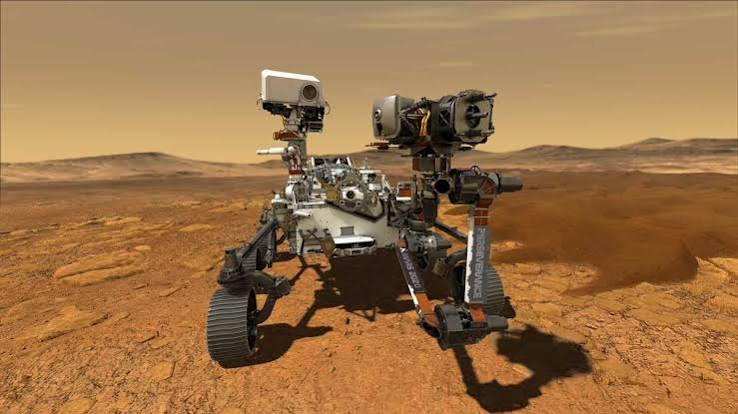
\includegraphics[height = 5cm]{images/perseverance_rover.jpg} }}%
    \caption*{Perseverance}
\end{figure}
\end{frame}

%Slide 1
\begin{frame}{Introduction} 
\begin{figure}
    \begin{columns}
        \only<1>{
        \column{.5\textwidth}
        \centering
        {{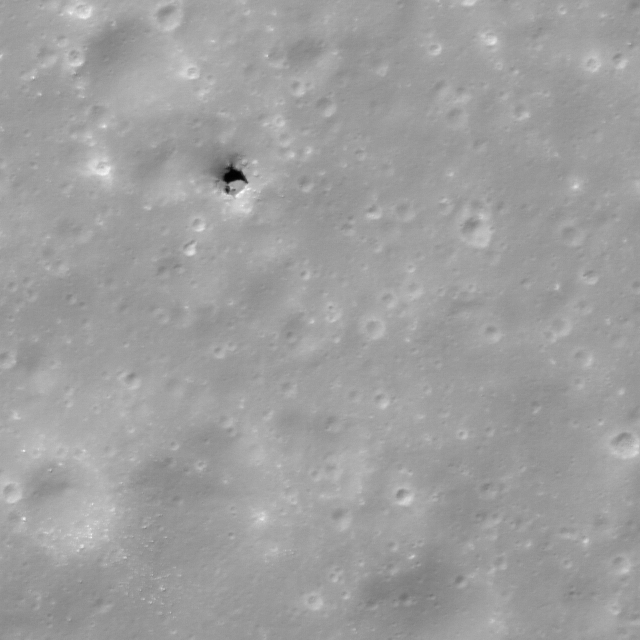
\includegraphics[height = 5cm]{images/m170118311rc_cropped.png} }}%
        \caption*{}
        }
        \only<2>{
        \column{.5\textwidth}
        \centering
        {{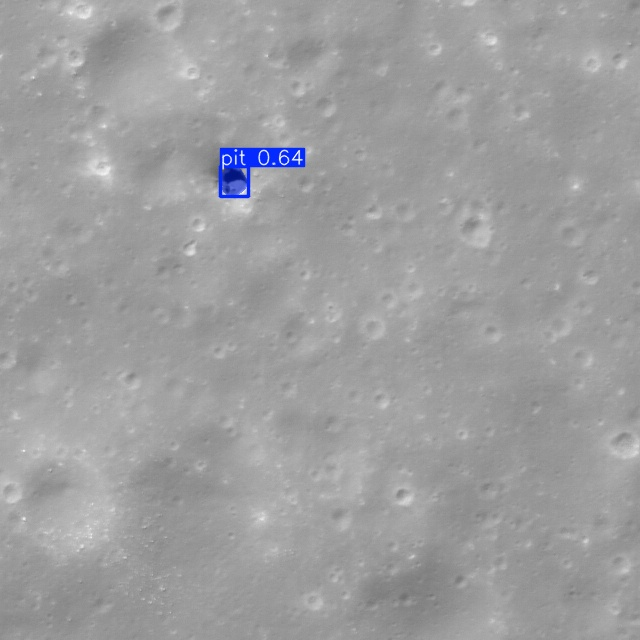
\includegraphics[height = 5cm]{images/m170118311rc_cropped.jpg} }}%
        \caption*{}
        }
    \end{columns}
\end{figure}
\end{frame}

%Slide 2
\begin{frame}{What are Lunar Skylights?}
\begin{figure}
    \begin{columns}
        \only<1,3>{
        \column{.5\textwidth}
        \centering
        {{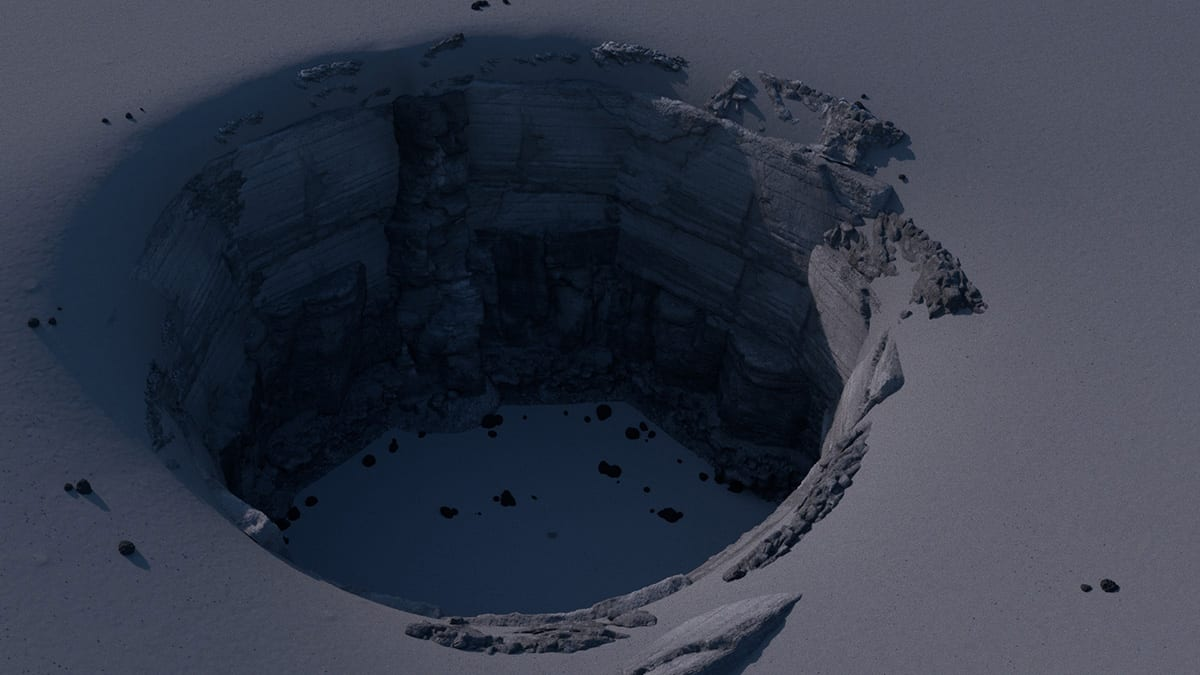
\includegraphics[height = 4cm]{images/lunar_skylight.jpg} }}%
        \caption*{skylight}
        }
        \only<2>{
        \column{.5\textwidth}
        \centering
        {{\includegraphics[height = 4cm]{images/Lava_river_cave_oregon.jpg} }}%
        \caption*{Oregon lava tube}
        }
        \only<2>{
        \column{.5\textwidth}
        \centering
        {{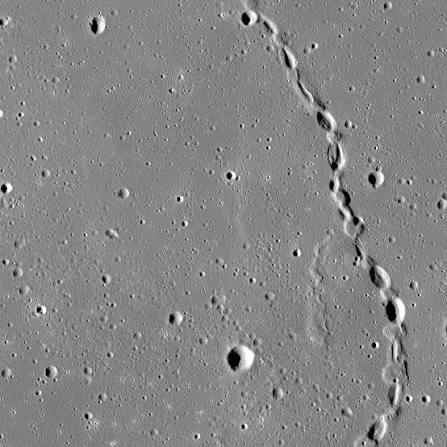
\includegraphics[height = 4cm]{images/lunar_lava_tube.jpg} }}%
        \caption*{Lunar lava tube}
        }
        \only<3>{
        \column{.5\textwidth}
        \centering
        {{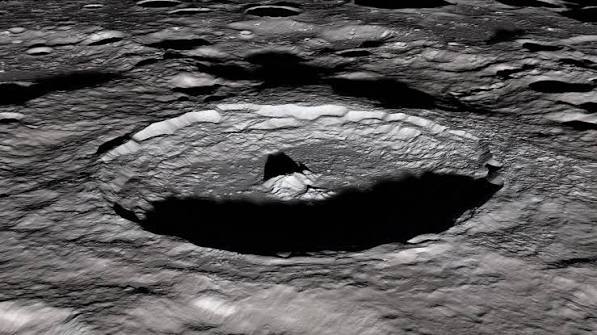
\includegraphics[height = 4cm]{images/crater.jpg} }}%
        \caption*{crater}
        }
    \end{columns}
\end{figure}
\end{frame}

\begin{frame}{Return to the Moon}
\begin{figure}
    \begin{columns}
        \only<1>{
        \column{.5\textwidth}
        \centering
        {{
\includegraphics[height = 5cm]{images/artemis.jpg} }}%
        }
        \only<2>{
        \column{.5\textwidth}
        \centering
        {{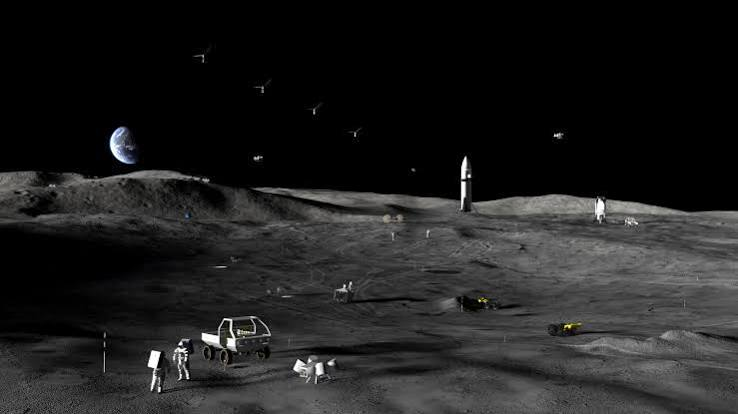
\includegraphics[height = 4.5cm]{images/lunar_base.jpg} }}%
        }
        \only<3>{
        \column{.5\textwidth}
        \centering
        {{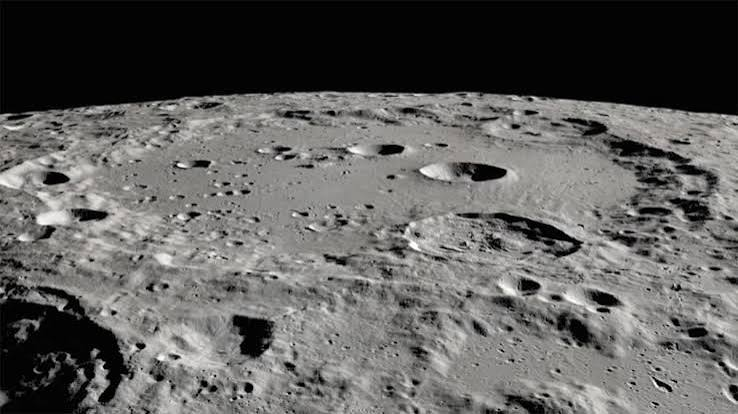
\includegraphics[height = 4cm]{images/lunar_surface.jpg} }}%
        }
        \only<3>{
        \column{.5\textwidth}
        \centering
        {{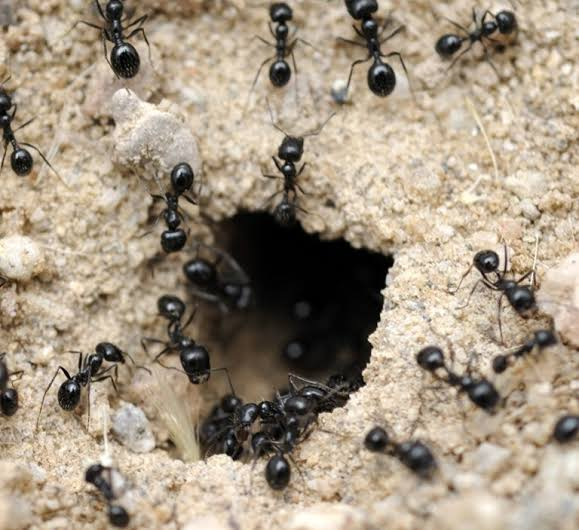
\includegraphics[height = 4cm]{images/ant_colony.jpg} }}%
        }
    \end{columns}
\end{figure}
\end{frame}

%Slide 3
\begin{frame}{Lunar Orbiter Narrow Angle Camera}
\begin{figure}
    \centering
    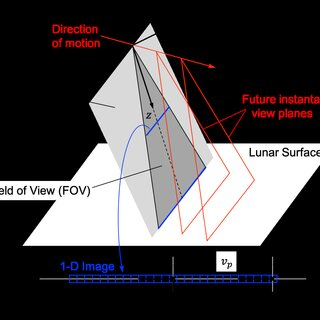
\includegraphics[height = 5cm]{images/pushbroom_camera.jpg}
    \caption*{Pushbroom camera}
\end{figure}
\end{frame}

%Slide 4
\begin{frame}{Downloading Images}
\begin{figure}
    \centering
    {{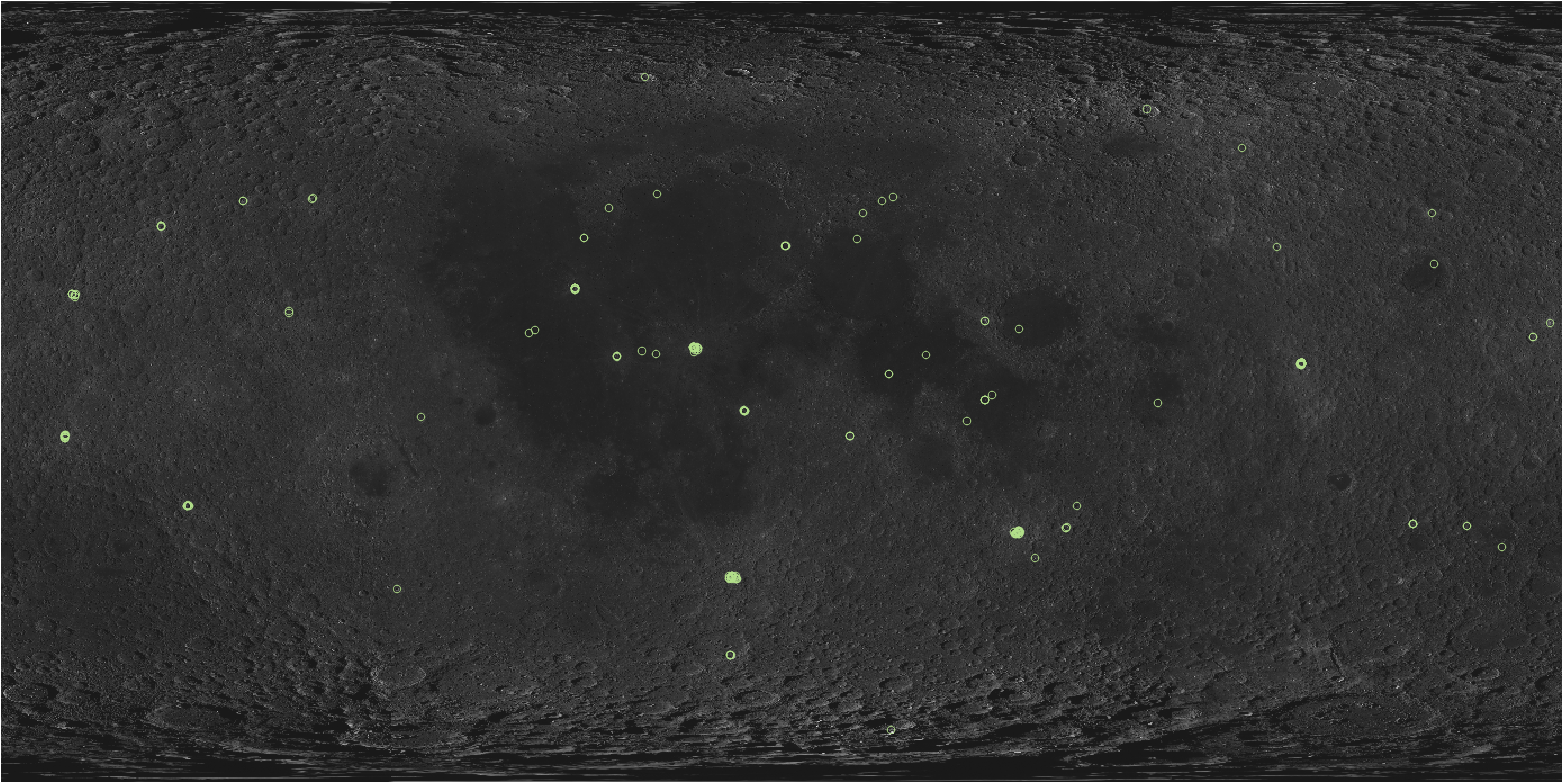
\includegraphics[height = 5cm]{images/LUNAR_PIT_LOCATIONS.png} }}%
    \caption*{Map of lunar pits}
\end{figure}
\end{frame}

%Slide 5
\begin{frame}{Cropping Images}
\begin{figure}
    \begin{columns}
        \column{0.5\textwidth}
        \centering
        {{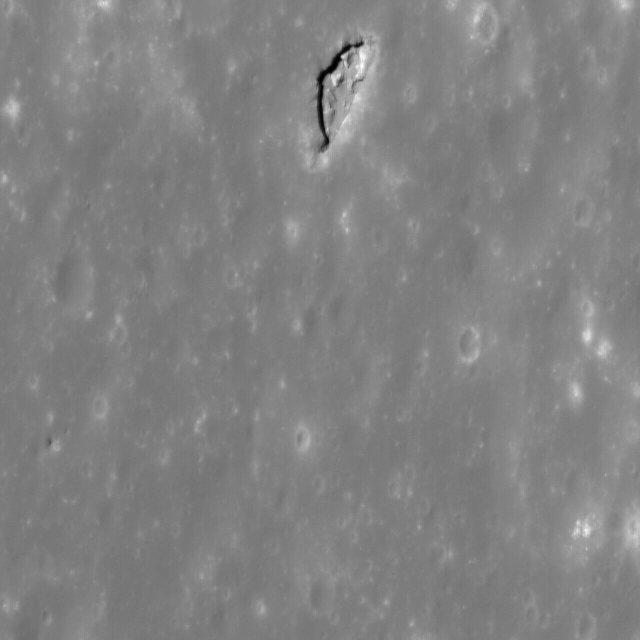
\includegraphics[height = 5cm]{images/m188378781lc_cropped.png} }}%
        \caption*{cropped with pit}
        
        \column{0.5\textwidth}
        \centering
        {{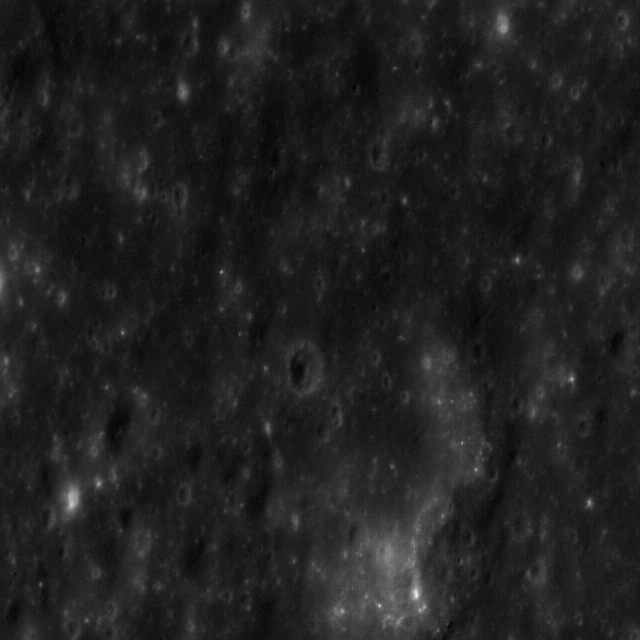
\includegraphics[height = 5cm]{images/m188378781lc_cropped_random.png} }}%
        \caption*{randomly cropped}
    \end{columns}
\end{figure}
\end{frame}

%Slide 5
\begin{frame}{Labeling Images}
\begin{figure}
    \begin{columns}
        \column{0.5\textwidth}
        \centering
        {{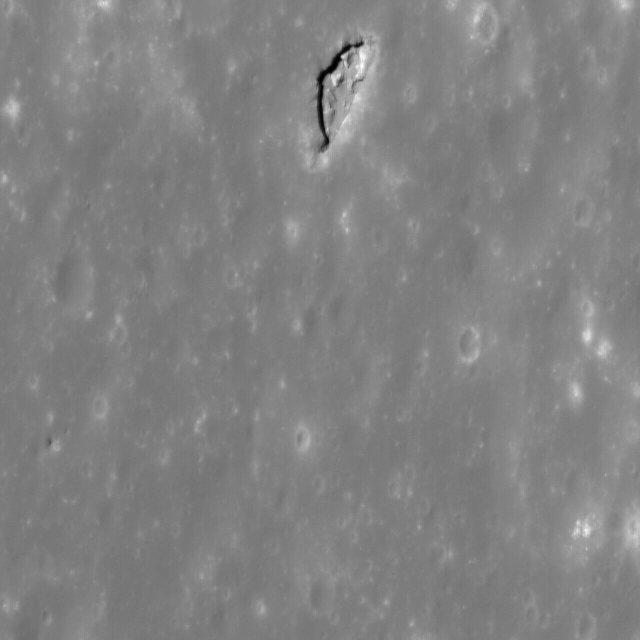
\includegraphics[height = 5cm]{images/m188378781lc_cropped.png} }}%
        \caption*{unmasked image}
        \column{0.5\textwidth}
        \centering
        {{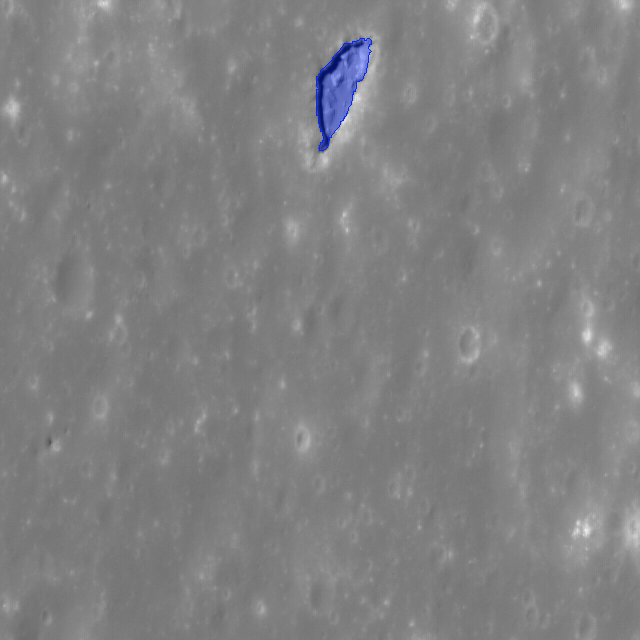
\includegraphics[height = 5cm]{m188378781lc_cropped_masked.png} }}%
        \caption*{masked image}
    \end{columns}
\end{figure}
\end{frame}

%Slide 5
\begin{frame}{Creating the Dataset}
\begin{figure}
    \begin{columns}
        \column{0.5\textwidth}
        \centering
        \begin{itemize}
            \item Train: 70\%
            \item Validation: 15\%
            \item Testing: 15\%
        \end{itemize}
        \column{0.5\textwidth}
        \centering
        {{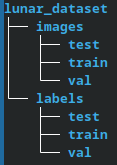
\includegraphics[height = 4cm]{images/lunar_dataset.png} }}%
        \caption*{Dataset}
    \end{columns}
\end{figure}
\end{frame}

%Slide 6
\begin{frame}{Training the Model}
\begin{figure}
    \centering
    {{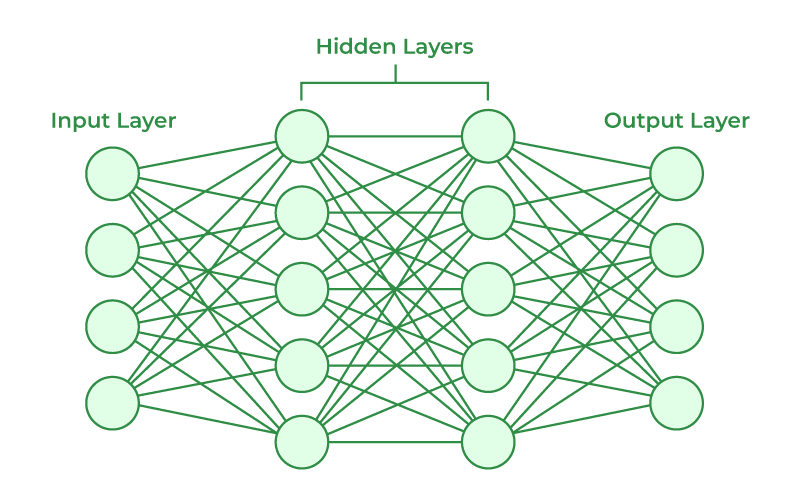
\includegraphics[height = 5cm]{images/Neural-Networks-Architecture.png} }}%
    \caption*{Neural network}
\end{figure}
\end{frame}

%Slide 7
\begin{frame}{You Only Look Once (YOLO)}
\begin{figure}
    \begin{columns}
        \column{0.5\textwidth}
        \centering
        {{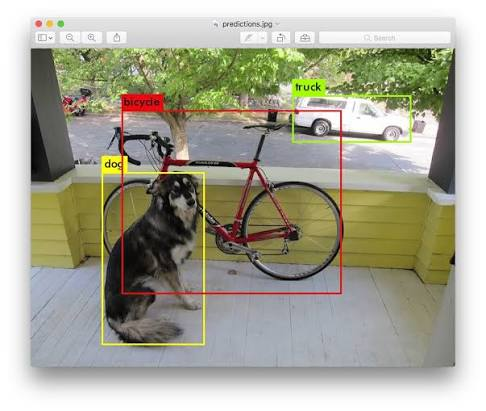
\includegraphics[height = 5cm]{images/yolo.jpg} }}%
        \caption*{YOLO Object Detection}
        \column{0.5\textwidth}
        \centering
        {{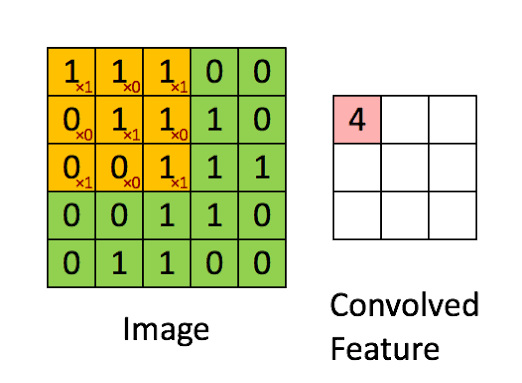
\includegraphics[height = 5cm]{images/convolutional_neural_network.png} }}%
        \caption*{Convolutional Neural Network}
    \end{columns}
\end{figure}
\end{frame}

%Slide 5
\begin{frame}{Model Accuracy}
    \begin{columns}
        \only<1>{    
            \begin{column}{0.5\textwidth}
                \centering
                {{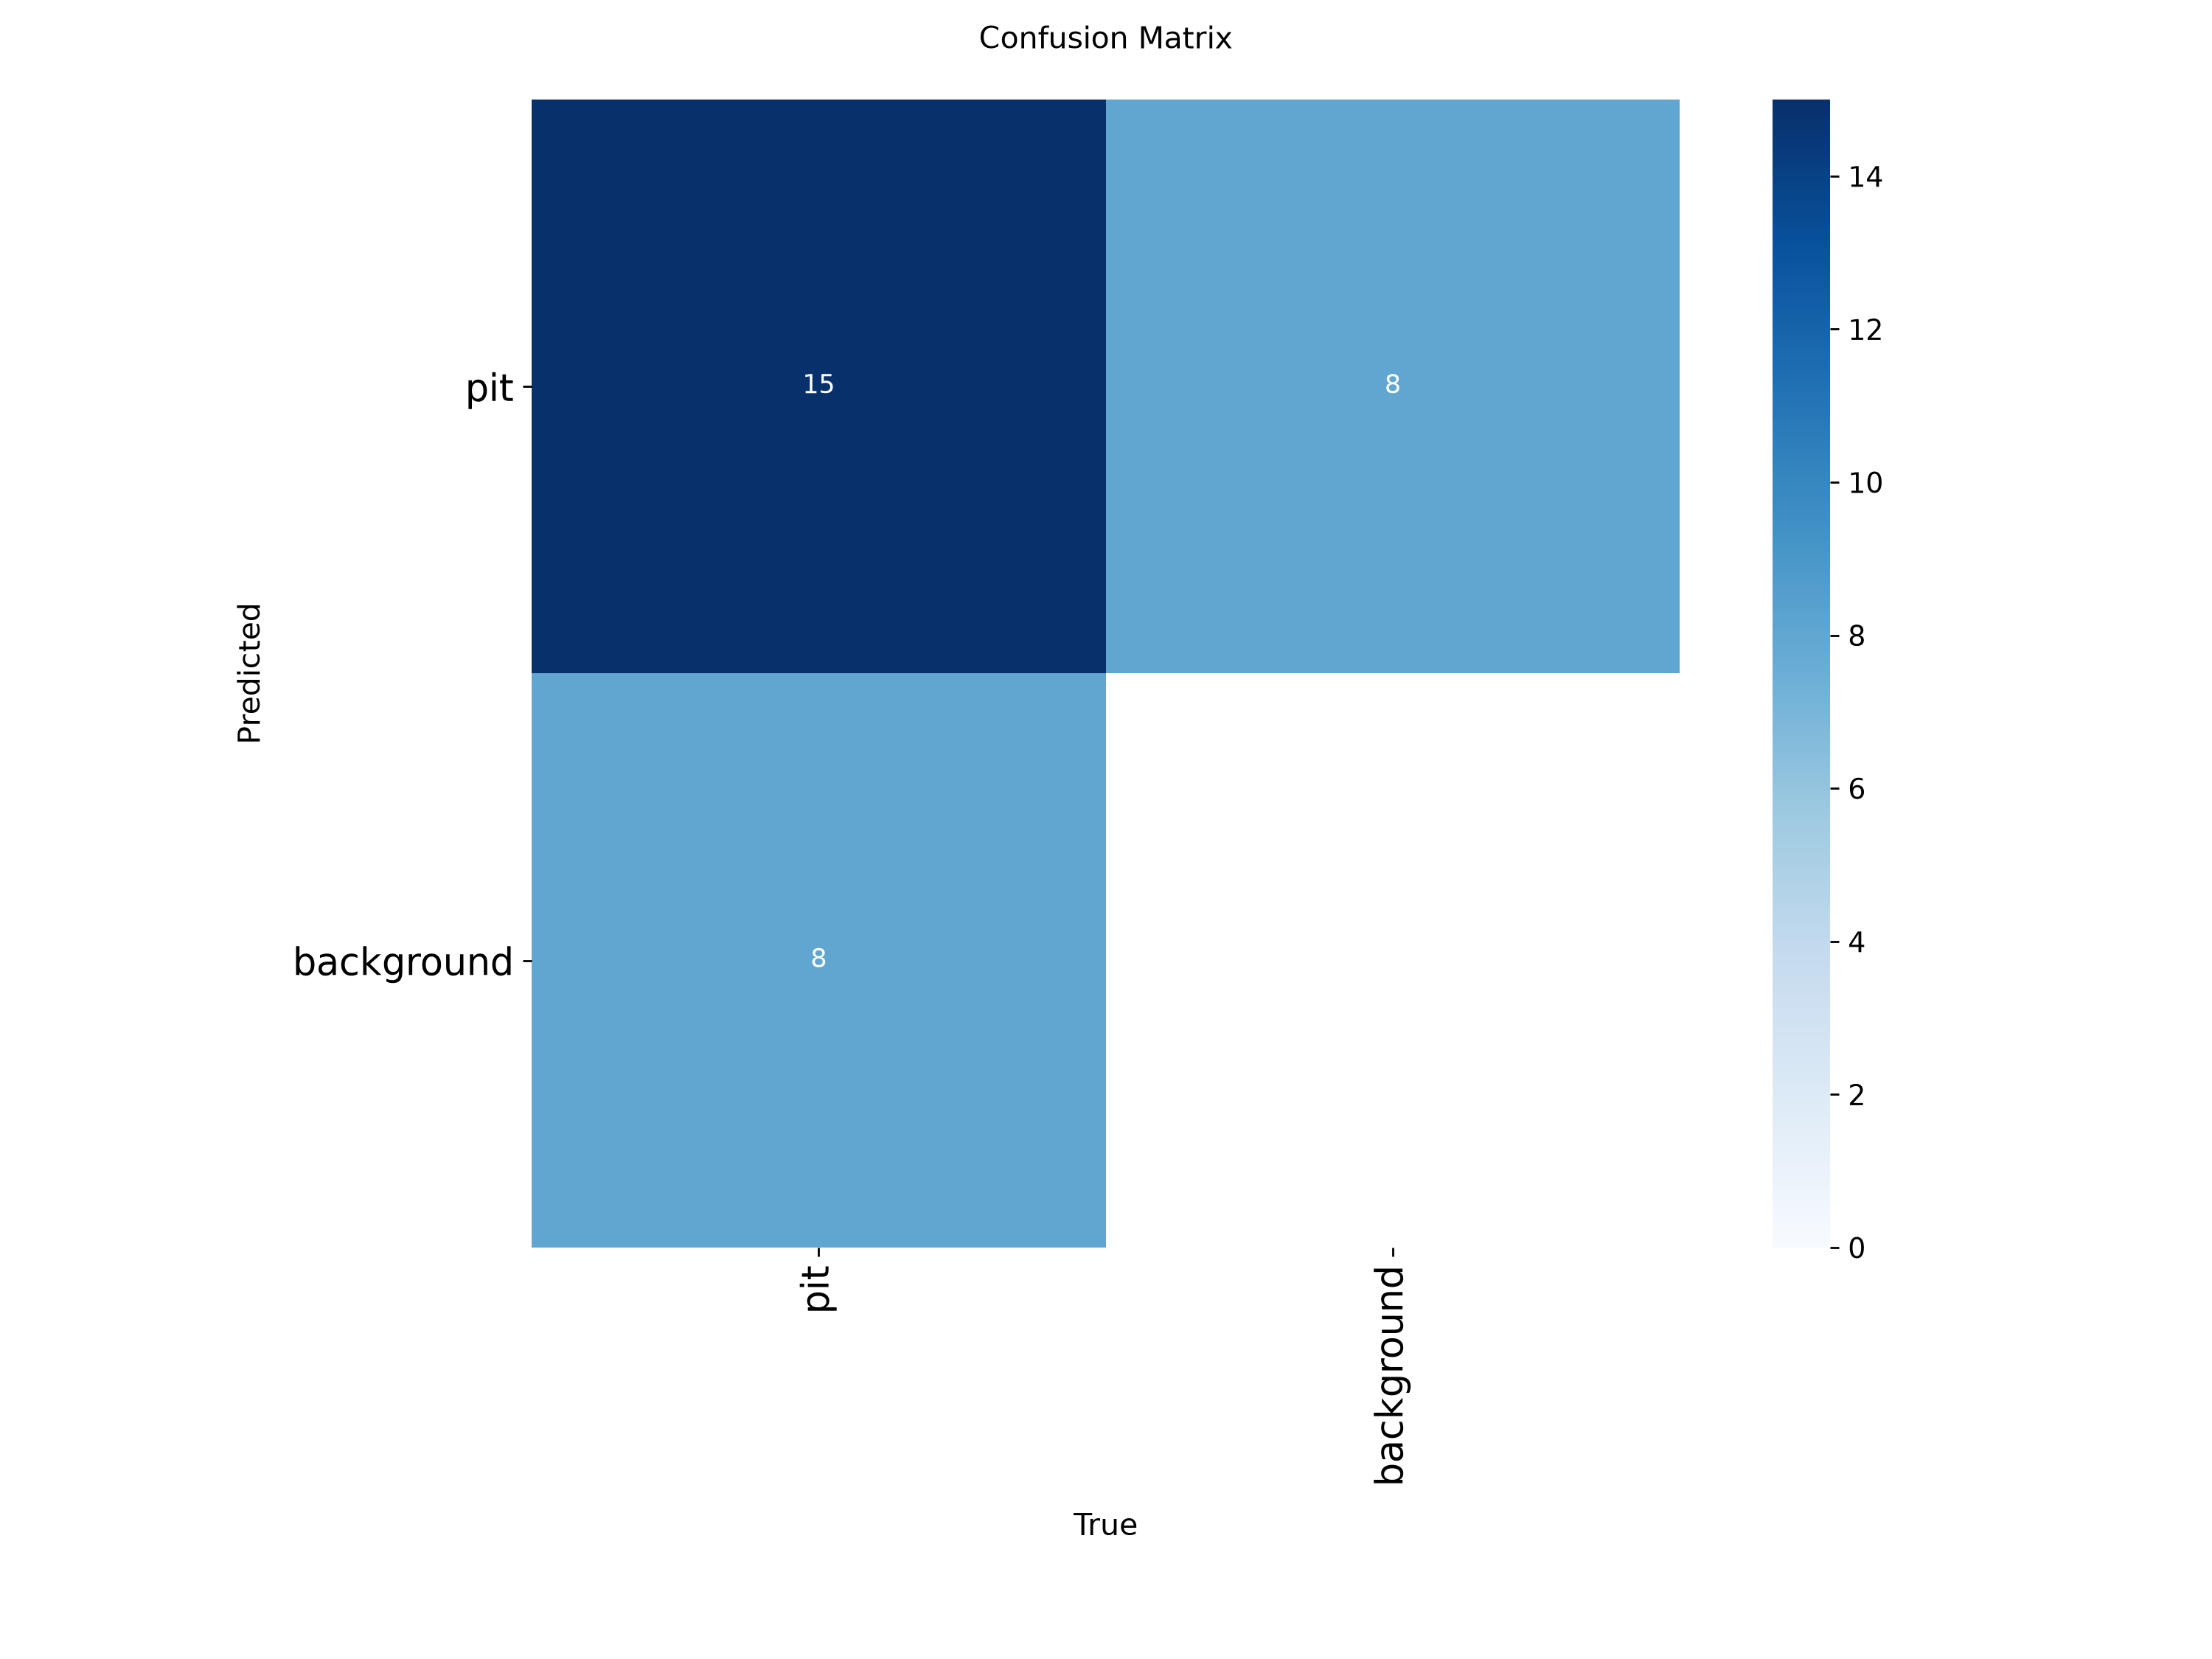
\includegraphics[height = 4cm]{images/confusion_matrix.png} }}%
                \captionof*{figure}{Confusion matrix}
            \end{column}
        }
        \only<1>{
            \begin{column}{0.5\textwidth}
                \centering
                {{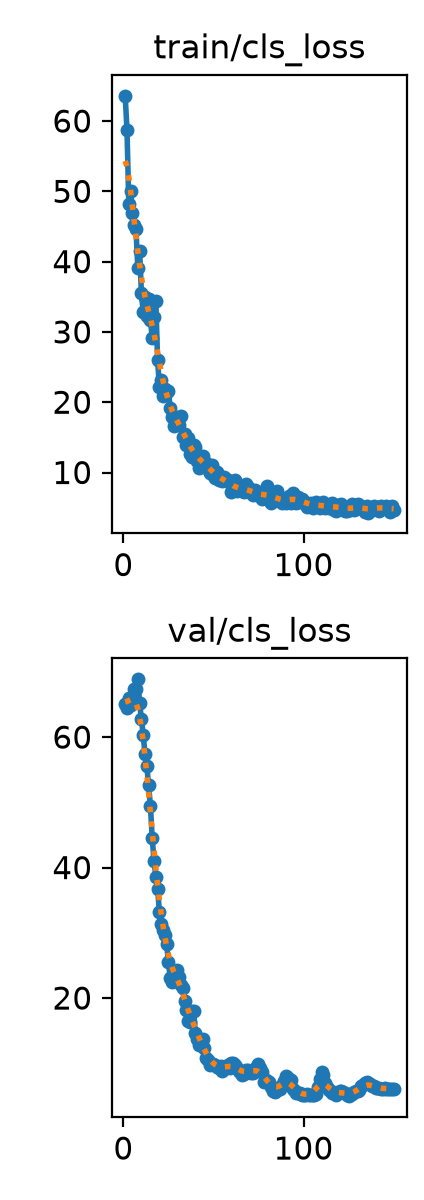
\includegraphics[width = 2cm]{images/class_loss.png} }}%
                \captionof*{figure}{Class loss}
            \end{column}
        }
        \only<2>{
            \begin{column}{0.5\textwidth}
                \centering
                {{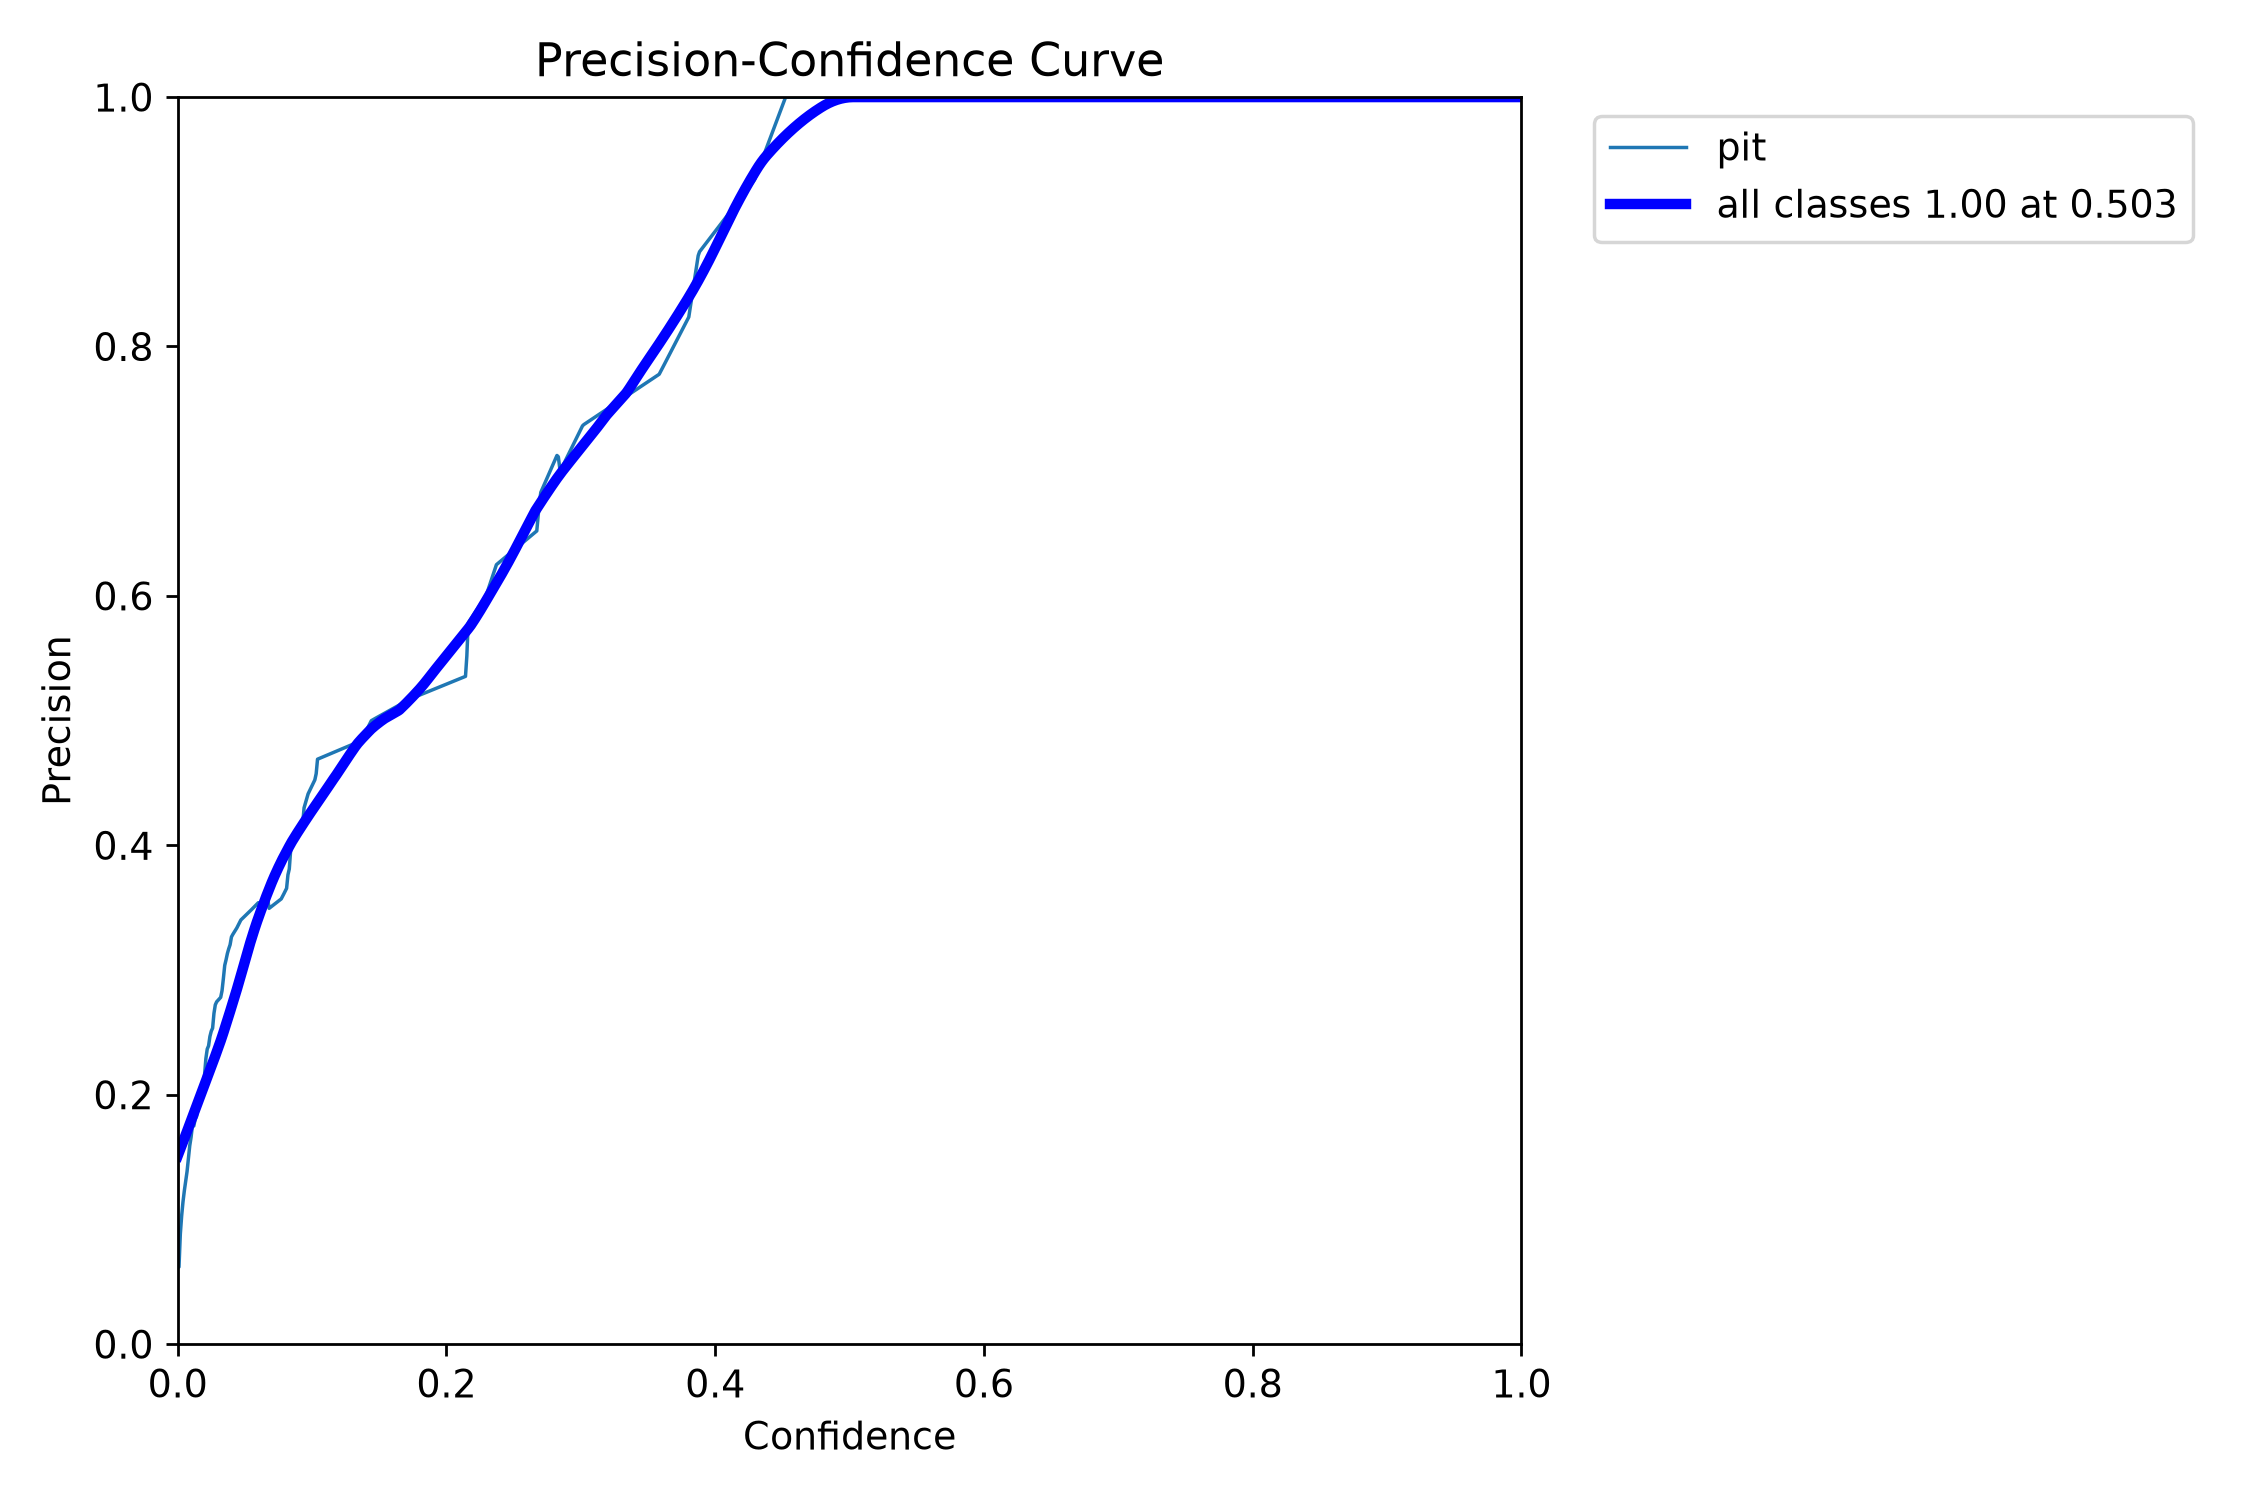
\includegraphics[height = 4cm]{images/BoxP_curve.png} }}%
                \captionof*{figure}{Precision vs Confidence}
            \end{column}
        }
        \only<2>{
            \begin{column}{0.5\textwidth}
                \centering
                {{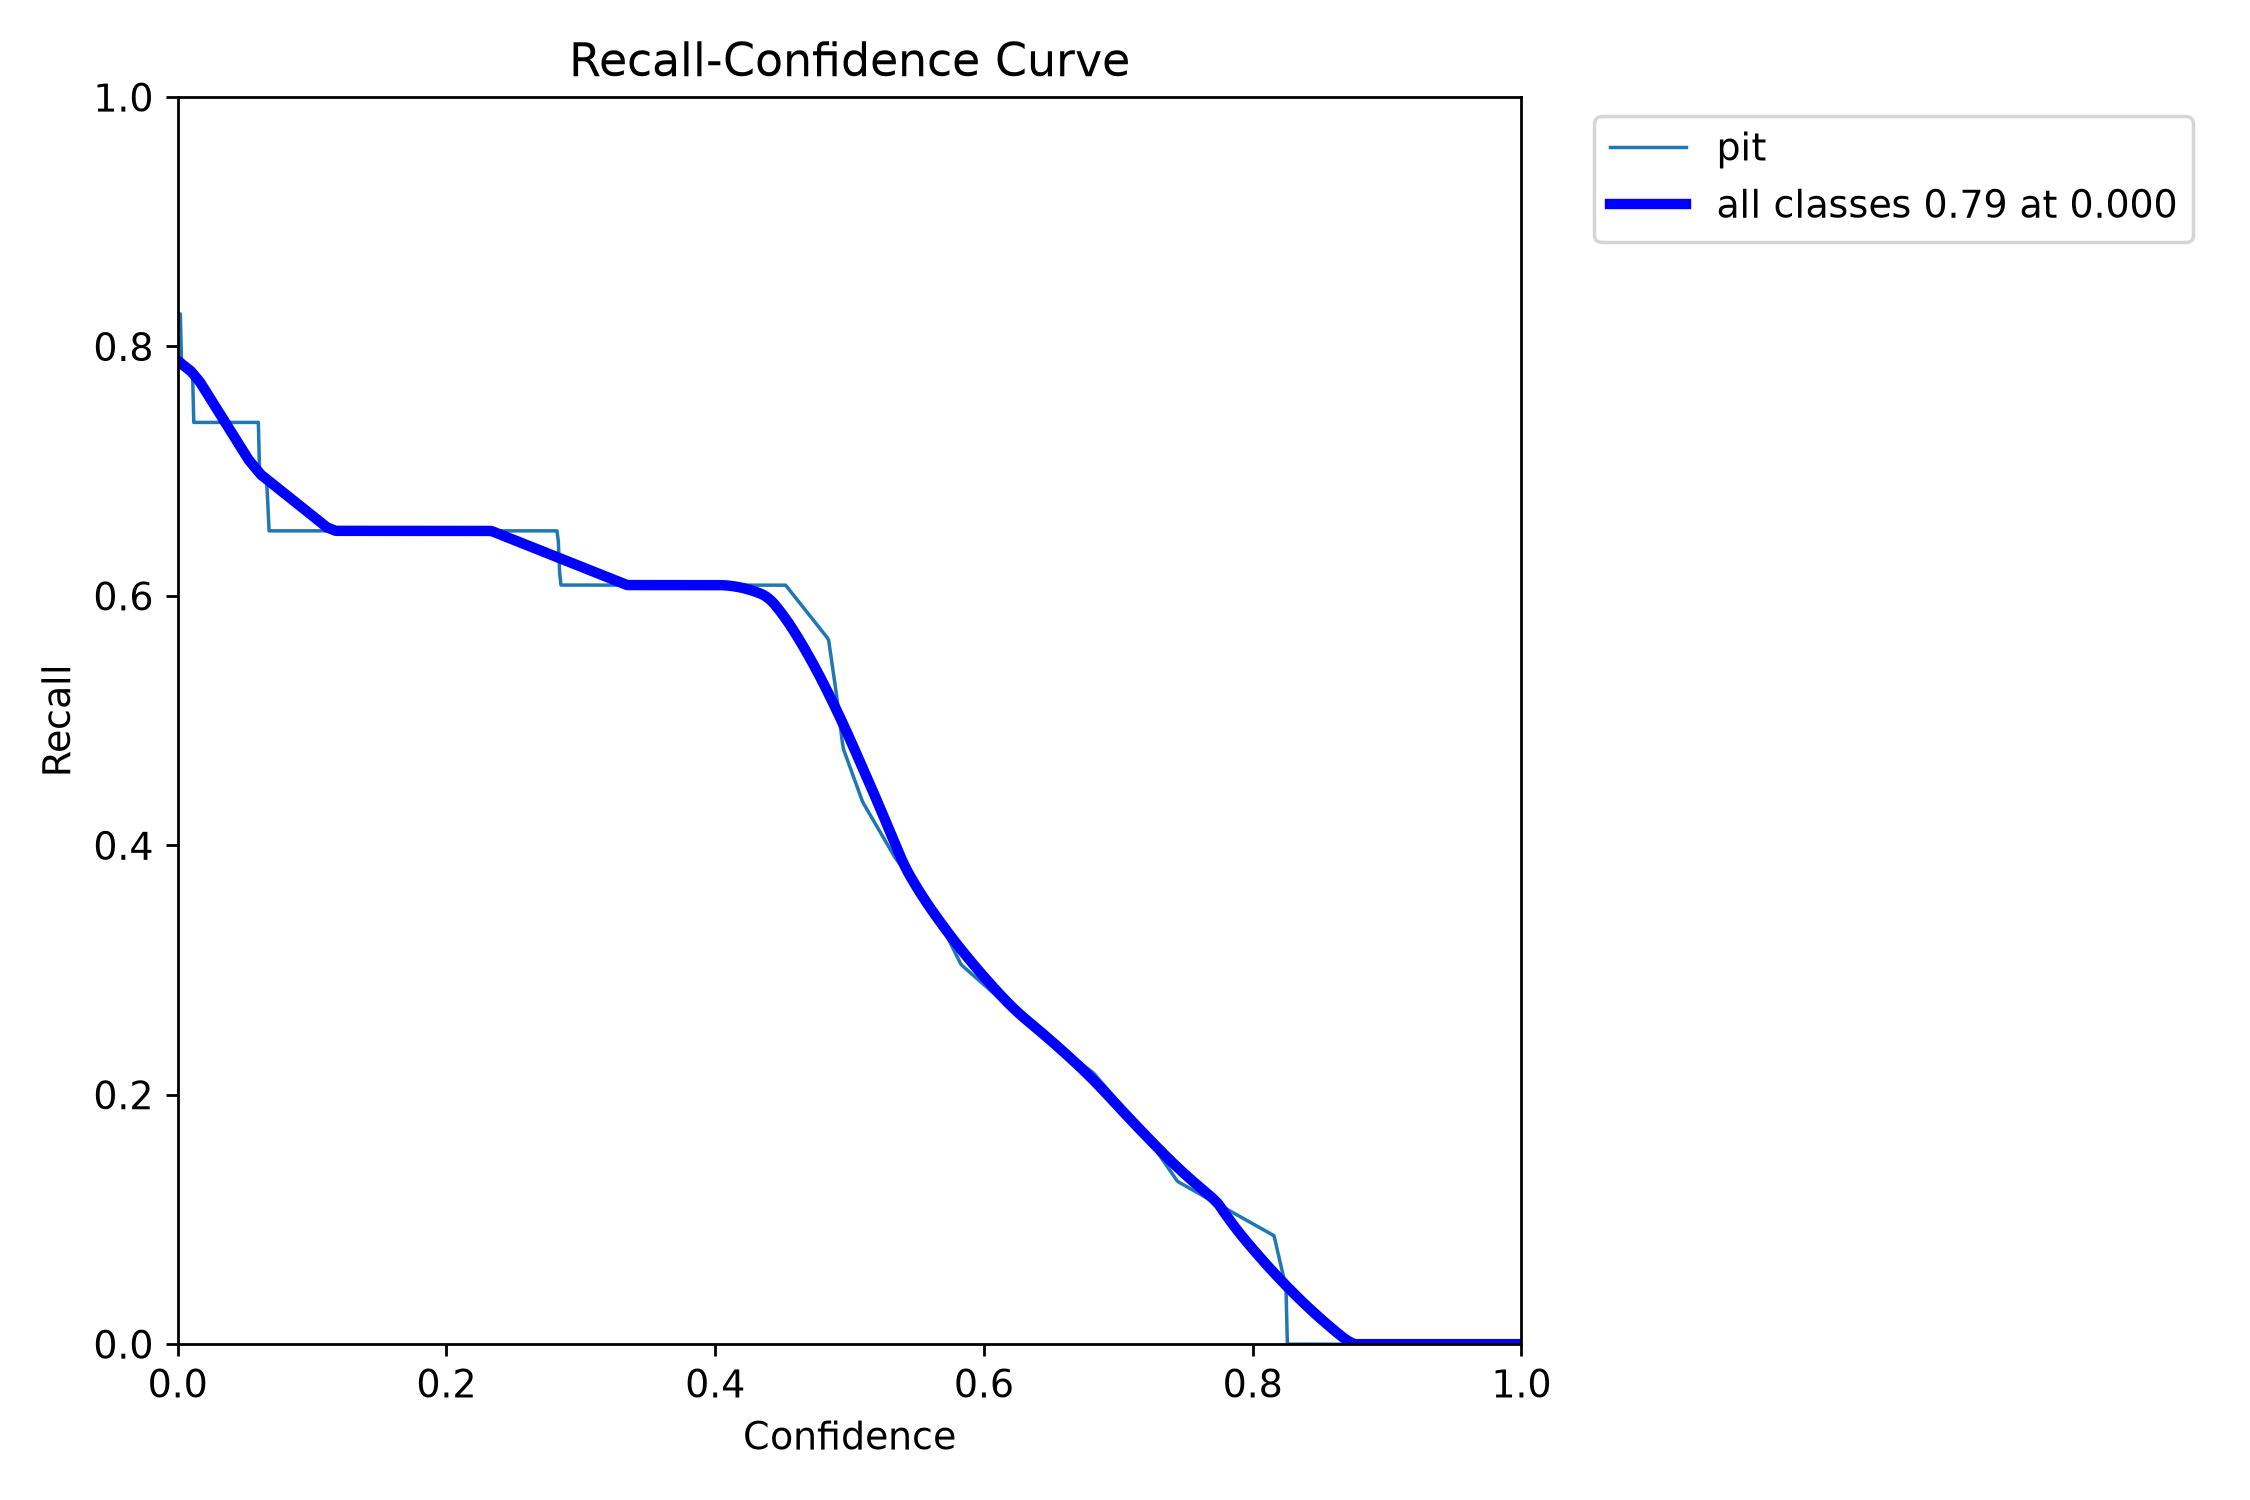
\includegraphics[height = 4cm]{images/BoxR_curve.png} }}%
                \captionof*{figure}{Recall vs Confidence}
            \end{column}
        }
    \end{columns}
\end{frame}

%Slide 8
\begin{frame}{Inferencing}
\begin{figure}
    \begin{columns}
        \only<1->{
            \column{0.5\textwidth}
                \centering
                {{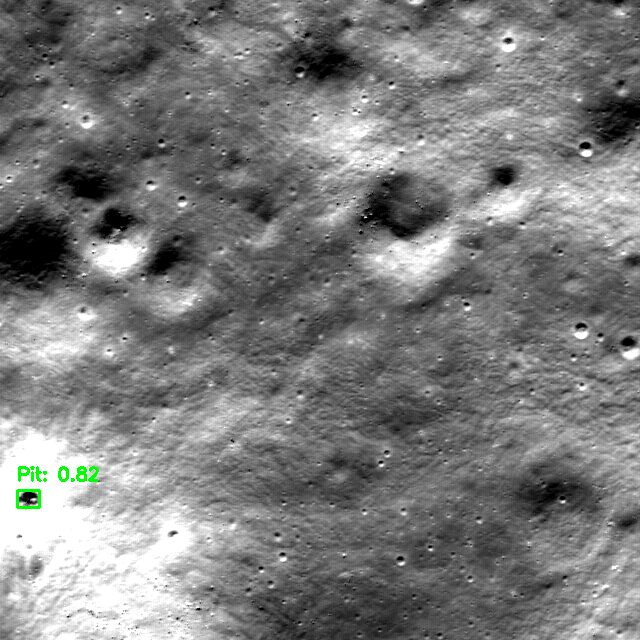
\includegraphics[height = 5cm]{M187722274LC_600_9600.png} }}%
                \caption*{Columns 2 \& 3}
        }
        \only<1>{
            \column{0.5\textwidth}
                \centering
                {{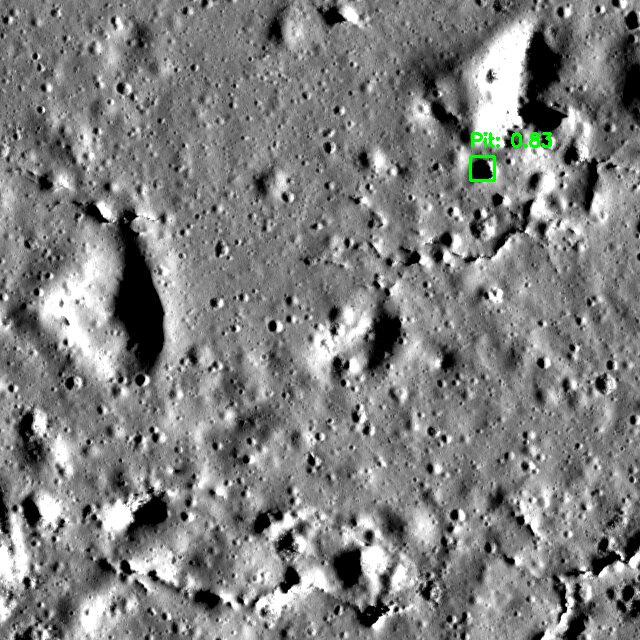
\includegraphics[height = 5cm]{images/M180387064LC_2400_19800.png} }}%
                \caption*{Columns 2 \& 3}
        }
        \only<2>{
            \column{0.5\textwidth}
                \centering
                {{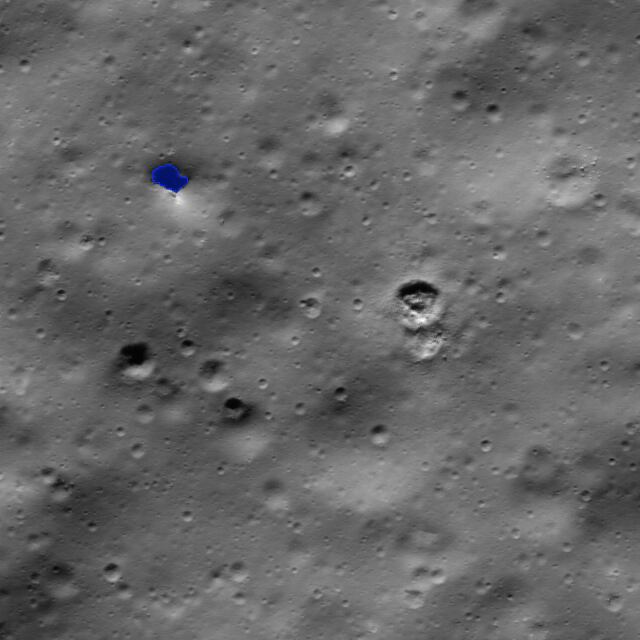
\includegraphics[height = 5cm]{images/m154705713rc_cropped_masked.png} }}%
                \caption*{Column 1}
        }
    \end{columns}
\end{figure}
\end{frame}

%Slide 5
\begin{frame}{Limitations}
\begin{figure}
    \begin{columns}
        \column{0.5\textwidth}
        \centering
        \begin{itemize}
            \item Not many identified pits to begin with
            \item Approx. $\frac{1}{3}$ of the catalog's images had coordinates
        \end{itemize}
        \column{0.5\textwidth}
        \centering
        {{
\includegraphics[height = 6cm]{images/metrics.png} }}%
        \caption*{Metrics}
    \end{columns}
\end{figure}
\end{frame}

%Slide 5
\begin{frame}{Conclusion}
\begin{figure}
    \begin{columns}
        \column{0.5\textwidth}
        \begin{itemize}
            \item Achieved initial goal
            \item Humans can quickly look through images
        \end{itemize}
        \column{0.5\textwidth}
        \centering
        {{
\includegraphics[height = 5cm]{images/magnifying_glass.jpg} }}%
        \caption*{}
    \end{columns}
\end{figure}
\end{frame}

\end{document}